\documentclass[a4paper,11pt]{book}
\usepackage{xeCJK}
\usepackage{amssymb}
\usepackage{graphicx}
\usepackage{amsmath}
\usepackage{amsfonts}
\usepackage{amsthm}
\usepackage{mathrsfs}
\usepackage{dsfont}
\usepackage{ifthen}
\usepackage{indentfirst}
\usepackage{enumerate}
\usepackage{color}
\usepackage{tikz}
\usetikzlibrary{arrows}
\usepackage[bf,small,indentafter,pagestyles]{titlesec}
\usepackage{titletoc}
\usepackage[top=1in, bottom=1in,left=0.8in,right=0.8in]{geometry}



\newtheorem{defi}{定义~}
\newtheorem{eg}{例~}
\newtheorem{ex}{~}
\newtheorem{rem}{注~}
\newtheorem{thm}{定理~}
\newtheorem{coro}{推论~}
\newtheorem{axiom}{公理~}
\newtheorem{prop}{性质~}

\setCJKmainfont[BoldFont=Adobe Heiti Std,ItalicFont=等线]{等线}

\newcommand{\onech}[4]{\par\begin{tabular}{p{.9\textwidth}}
		A.~#1\\
		B.~#2\\
		C.~#3\\
		D.~#4
	\end{tabular}}
	
\newcommand{\twoch}[4]{\par\begin{tabular}{p{.46\textwidth}p{.46\textwidth}}
			A.~#1& B.~#2\\
			C.~#3& D.~#4
		\end{tabular}}
		
\newcommand{\vartwoch}[4]{\par\begin{tabular}{p{.46\textwidth}p{.46\textwidth}}
				(1)~#1& (2)~#2\\
				(3)~#3& (4)~#4
			\end{tabular}}
			
			
\newcommand{\fourch}[4]{\par\begin{tabular}{p{.23\textwidth}p{.23\textwidth}p{.23\textwidth}p{.23\textwidth}}
					A.~#1 &B.~#2& C.~#3& D.~#4
				\end{tabular}}
				
\newcommand{\varfourch}[4]{\par\begin{tabular}{p{.23\textwidth}p{.23\textwidth}p{.23\textwidth}p{.23\textwidth}}
						(1)~#1 &(2)~#2& (3)~#3& (4)~#4
					\end{tabular}}
					
				

\newcommand{\blank}[1]{\underline{\hbox to #1pt{}}}
\newcommand{\bracket}[1]{(\hbox to #1pt{})}

\newcommand{\vct}{\overrightarrow}


\renewcommand{\baselinestretch}{1.5}

\begin{document}
	\section{集合、命题、不等式}
	
	\subsection{集合及相关知识}
	
	\begin{ex}
		设全集是实数集$\mathbf{R}$, $M=\{x|-2\le x\le 2\}$, $N=\{x|x<1\}$, 则$\complement_UM\cap N$等于\blank{60}.
	\end{ex}
	
	
	\begin{ex}
		如图, 在平面直角坐标系中, $\Omega$是一个与$x$轴的正半轴, $y$轴的正半轴分别相切于点$C$、$D$的定圆所围成的区域(含边界). $A$、$B$、$C$、$D$是该圆的四等分点. 若点$P(x,y)$、$P'(x',y')$满足$x\le x'$且$y\ge y'$, 则称$P$优于$P'$. 如果$\Omega$中的点$Q$满足: 不存在$\Omega$中的其它点优于$Q$, 那么所有这样的点$Q$组成的集合是劣弧\blank{15}.
		\begin{center}
			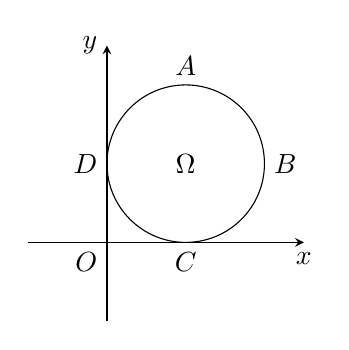
\begin{tikzpicture}[>=stealth]
			\draw [->] (-1,0) -- (0,0) node [below left] {$O$} -- (2.5,0) node [below] {$x$};
			\draw [->] (0,-1) -- (0,2.5) node [left] {$y$};
			\draw (1,1) node {$\Omega$} circle (1);
			\draw (1,0) node [below] {$C$} (2,1) node [right] {$B$} (1,2) node [above] {$A$} (0,1) node [left] {$D$};
			\end{tikzpicture}
		\end{center}
		\fourch{$AB$}{$BC$}{$CD$}{$DA$}
	\end{ex}
	
	\begin{ex}
		设$A=\{x|x^2+px+15=0\}$, $B=\{x|x^2-5x+q=0\}$, 且$A\cap B=\{3\}$, 则$p=$\blank{30}, $q=$\blank{30}, $A\cup B=$\blank{30}.
	\end{ex}
\end{document}